\documentclass[conference,a4paper,twoside]{IEEEtran}
\usepackage[utf8]{inputenc}
\usepackage{amsmath}
\usepackage{amsfonts}
\usepackage{amssymb}
\usepackage{graphicx}
\usepackage{url}
\usepackage{hyperref}
\RequirePackage[date=terse,isbn=true,doi=true,url=false,maxbibnames=9,backref=false,backend=bibtex]{biblatex}
\addbibresource{securityupdates.bib}
\renewcommand{\bibfont}{\small}

\AtEveryBibitem{% Clean up the bibtex rather than editing it
 \clearname{editor} % remove editors
}

\author{Daniel R.\ Thomas, Daniel T.\ Wagner, Alastair R.\ Beresford and Andrew Rice}

\newcommand{\daNumSigModels}{18}
\newcommand{\daSigNumDevices}{100}
\newcommand{\daSigNumDeviceDays}{10\,000}
\newcommand{\daSigNumDays}{100}
\newcommand{\daSigNumDevicesDay}{20}
\newcommand{\daSigVersionPerc}{1\%}
\newcommand{\daSigVersionDays}{10}
\newcommand{\daNumVulnsUsed}{11}
\newcommand{\daNumDeviceDataDevices}{50}
\newcommand{\daOSYearsOfData}{4}
\newcommand{\daOSMonthsOfData}{51}
\newcommand{\daStartDate}{2011-07-01}
\newcommand{\daEndDate}{2015-09-22}
\newcommand{\daFullDeployedAt}{95\%}
\newcommand{\daNumManufacturers}{302}
\newcommand{\daNumSigManufacturers}{10}
\newcommand{\daNumModels}{2\,770}
\newcommand{\daNumOperators}{1\,470}
\newcommand{\daNumSigOperators}{14}
\newcommand{\daNumOSDevices}{20\,500}
\newcommand{\daOSVersionPercValidLines}{99.9\%}
\newcommand{\daOSTotalDaysData}{1\,350\,000}
\newcommand{\daMeanInsecurityPercNominal}{87.3\%}
\newcommand{\daMeanInsecurityPerc}{$87.3 \pm 0.0\%$}
\newcommand{\daMeanInsecurityPercTwosfNominal}{87\%}
\newcommand{\daMeanInsecurityPercTwosf}{$87 \pm 0\%$}
\newcommand{\daMeanSecurityPercNominal}{12.7\%}
\newcommand{\daMeanSecurityPerc}{$12.7 \pm 0.0\%$}
\newcommand{\daMeanSecurityPercTwosfNominal}{13\%}
\newcommand{\daMeanSecurityPercTwosf}{$13 \pm 0\%$}
\newcommand{\daVulnFreeNominal}{0.127}
\newcommand{\daVulnFree}{$0.127 \pm 0.0$}
\newcommand{\daMeanOutstandingVulnerabilities}{$0.509 \pm 0.0$}
\newcommand{\daUpdatednessNominal}{0.0553}
\newcommand{\daUpdatedness}{$0.0553 \pm 0.0$}
\newcommand{\daUpdatednessPercNominal}{5.53\%}
\newcommand{\daUpdatednessPerc}{$5.53 \pm 0.0\%$}
\newcommand{\daUpdatednessPercTwosfNominal}{5.5\%}
\newcommand{\daUpdatednessPercTwosf}{$5.5 \pm 0.0\%$}
\newcommand{\daSecurityScoreNominal}{2.93}
\newcommand{\daSecurityScore}{$2.93 \pm 0.0$}
\newcommand{\daCurrentMeanInsecurityPercNominal}{68.8\%}
\newcommand{\daCurrentMeanInsecurityPerc}{$68.8 \pm 0.0\%$}
\newcommand{\daCurrentMeanInsecurityPercTwosfNominal}{69\%}
\newcommand{\daCurrentMeanInsecurityPercTwosf}{$69 \pm 0\%$}
\newcommand{\daCurrentMeanSecurityPercNominal}{31.2\%}
\newcommand{\daCurrentMeanSecurityPerc}{$31.2 \pm 0.2\%$}
\newcommand{\daCurrentMeanSecurityPercTwosfNominal}{31\%}
\newcommand{\daCurrentMeanSecurityPercTwosf}{$31 \pm 0\%$}
\newcommand{\daCurrentVulnFreeNominal}{0.312}
\newcommand{\daCurrentVulnFree}{$0.312 \pm 0.002$}
\newcommand{\daCurrentMeanOutstandingVulnerabilities}{$0.0645 \pm 0.0$}
\newcommand{\daCurrentUpdatednessNominal}{0.0934}
\newcommand{\daCurrentUpdatedness}{$0.0934 \pm 0.0019$}
\newcommand{\daCurrentUpdatednessPercNominal}{9.34\%}
\newcommand{\daCurrentUpdatednessPerc}{$9.34 \pm 0.19\%$}
\newcommand{\daCurrentUpdatednessPercTwosfNominal}{9.3\%}
\newcommand{\daCurrentUpdatednessPercTwosf}{$9.3 \pm 0.0\%$}
\newcommand{\daCurrentSecurityScoreNominal}{4.43}
\newcommand{\daCurrentSecurityScore}{$4.43 \pm 0.0$}
\newcommand{\daDailyParticipationNominal}{872}
\newcommand{\daDailyParticipation}{$872 \pm 271$}
\newcommand{\daNumFullVersions}{1\,300}
\newcommand{\daNumSigFullVersions}{101}
\newcommand{\daNumOSVersions}{50}
\newcommand{\daNumSigOSVersions}{28}
\newcommand{\daNumAPIVersions}{16}
\newcommand{\daNumFullVersionUpdates}{4\,670}
\newcommand{\daNumOSVersionUpdates}{3\,940}
\newcommand{\daUpdatesPerYearNominal}{1.27}
\newcommand{\daUpdatesPerYear}{$1.27 \pm 0.01$}
\newcommand{\daUpdatesPerYearTwosfNominal}{1.3}
\newcommand{\daUpdatesPerYearTwosf}{$1.3 \pm 0.0$}
\newcommand{\daNumFullOnlyVersionUpdates}{724}
\newcommand{\daNumSecurityUpdates}{1\,270}
\newcommand{\daNumPossibleSecurityUpdates}{2\,310}
\newcommand{\daOSCurveFitParamFirst}{83.6}
\newcommand{\daOSCurveFitParamSecond}{\num{0.0028}}
\newcommand{\daOSCurveFitRMSE}{0.114}
\newcommand{\daOSCurvePolyRMSE}{0.114}
\newcommand{\daOSCurveSplineRMSE}{0.114}
\newcommand{\daOSCurveHalfDeployedYearsNominal}{0.908}
\newcommand{\daOSCurveHalfDeployedYears}{$0.908 \pm 0.254$}
\newcommand{\daOSCurveHalfDeployedNominal}{332}
\newcommand{\daOSCurveHalfDeployed}{$332 \pm 92$}
\newcommand{\daOSCurveFullDeployedYearsNominal}{3.16}
\newcommand{\daOSCurveFullDeployedYears}{$3.16 \pm 72$}
\newcommand{\daOSCurveFullDeployedNominal}{1\,150}
\newcommand{\daOSCurveFullDeployed}{$1\,150 \pm 265\,000$}
\newcommand{\daAPICurveFitParamFirst}{97.8}
\newcommand{\daAPICurveFitParamSecond}{\num{0.0028}}
\newcommand{\daAPICurveFitRMSE}{0.11}
\newcommand{\daAPICurvePolyRMSE}{0.111}
\newcommand{\daAPICurveSplineRMSE}{0.111}
\newcommand{\daAPICurveHalfDeployedYearsNominal}{0.946}
\newcommand{\daAPICurveHalfDeployedYears}{$0.946 \pm 0.244$}
\newcommand{\daAPICurveHalfDeployedNominal}{345}
\newcommand{\daAPICurveHalfDeployed}{$345 \pm 89$}
\newcommand{\daAPICurveFullDeployedYearsNominal}{3.2}
\newcommand{\daAPICurveFullDeployedYears}{$3.2 \pm 7$}
\newcommand{\daAPICurveFullDeployedNominal}{1\,170}
\newcommand{\daAPICurveFullDeployed}{$1\,170 \pm 265\,000$}
\newcommand{\daVulnAPKDuplicateFileOctoberPerc}{91.7\%}
\newcommand{\daVulnZergRushMonthsDefFixDeployed}{27.3}
\newcommand{\daTabSecScoresmanufacturer}{\begin{table*} \centering \begin{tabular}{l|c|c|c|c} Name & $f$ & $u$ & $m$ & \textbf{score} \\ &&&& (out of 10) \\ \hline LG & $0.24 \pm 0.00$ & $0.34 \pm 0.00$ & $0.60 \pm 0.01$ & $4.11 \pm 0.02$ \\  Motorola & $0.19 \pm 0.00$ & $0.12 \pm 0.00$ & $0.71 \pm 0.02$ & $3.11 \pm 0.02$ \\  Samsung & $0.13 \pm 0.00$ & $0.04 \pm 0.00$ & $0.58 \pm 0.00$ & $2.80 \pm 0.00$ \\  Sony & $0.14 \pm 0.00$ & $0.19 \pm 0.00$ & $1.09 \pm 0.02$ & $2.66 \pm 0.02$ \\  HTC & $0.14 \pm 0.00$ & $0.10 \pm 0.00$ & $0.86 \pm 0.01$ & $2.65 \pm 0.02$ \\  asus & $0.21 \pm 0.00$ & $0.51 \pm 0.01$ & $6.01 \pm 0.07$ & $2.38 \pm 0.02$ \\  other & $0.06 \pm 0.00$ & $0.05 \pm 0.00$ & $1.00 \pm 0.01$ & $2.02 \pm 0.02$ \\  alps & $0.03 \pm 0.00$ & $0.19 \pm 0.01$ & $3.99 \pm 0.08$ & $0.80 \pm 0.02$ \\  Symphony & $0.00 \pm 0.00$ & $0.09 \pm 0.00$ & $5.00 \pm 0.05$ & $0.32 \pm 0.01$ \\  walton & $0.00 \pm 0.00$ & $0.09 \pm 0.00$ & $6.00 \pm 0.08$ & $0.27 \pm 0.01$ \\ \end{tabular} \caption{Security scores for manufacturers} \label{tab:sec_manufacturer} \end{table*}}
\newcommand{\daSecScoreBestmanufacturer}{LG}
\newcommand{\daSecScoreBestmanufacturerScoreNominal}{4.11}
\newcommand{\daSecScoreBestmanufacturerScore}{$4.11 \pm 0.0$}
\newcommand{\daSecScoreBestmanufacturerNumFullVersions}{142}
\newcommand{\daSecScoreWorstmanufacturer}{walton}
\newcommand{\daSecScoreWorstmanufacturerScoreNominal}{0.273}
\newcommand{\daSecScoreWorstmanufacturerScore}{$0.273 \pm 0.007$}
\newcommand{\daSecScoreWorstmanufacturerNumFullVersions}{21}
\newcommand{\daTabSecScoresmodel}{\begin{table*} \centering \begin{tabular}{l|c|c|c|c} Name & $f$ & $u$ & $m$ & \textbf{score} \\ &&&& (out of 10) \\ \hline Galaxy Nexus & $0.50 \pm 0.00$ & $0.54 \pm 0.01$ & $1.53 \pm 0.04$ & $4.70 \pm 0.04$ \\  Nexus 4 & $0.33 \pm 0.00$ & $0.82 \pm 0.01$ & $6.06 \pm 0.09$ & $3.78 \pm 0.04$ \\  Nexus 7 & $0.27 \pm 0.00$ & $0.73 \pm 0.01$ & $5.92 \pm 0.09$ & $3.29 \pm 0.04$ \\  other & $0.10 \pm 0.00$ & $0.14 \pm 0.00$ & $0.51 \pm 0.00$ & $3.08 \pm 0.00$ \\  Desire HD & $0.08 \pm 0.00$ & $0.05 \pm 0.00$ & $0.38 \pm 0.02$ & $2.91 \pm 0.04$ \\  HTC Sensation & $0.35 \pm 0.00$ & $0.01 \pm 0.01$ & $1.57 \pm 0.05$ & $2.44 \pm 0.05$ \\  GT-I9100 & $0.22 \pm 0.00$ & $0.02 \pm 0.00$ & $1.23 \pm 0.02$ & $2.27 \pm 0.02$ \\  HTC Desire S & $0.02 \pm 0.00$ & $0.02 \pm 0.00$ & $1.00 \pm 0.06$ & $1.74 \pm 0.07$ \\  GT-N7000 & $0.25 \pm 0.00$ & $0.00 \pm 0.00$ & $2.52 \pm 0.05$ & $1.43 \pm 0.02$ \\  GT-P1000 & $0.01 \pm 0.00$ & $0.00 \pm 0.01$ & $1.79 \pm 0.06$ & $0.90 \pm 0.05$ \\  GT-I9505 & $0.06 \pm 0.00$ & $0.13 \pm 0.00$ & $6.82 \pm 0.07$ & $0.62 \pm 0.01$ \\  GT-I9300 & $0.13 \pm 0.00$ & $0.01 \pm 0.00$ & $6.23 \pm 0.04$ & $0.57 \pm 0.01$ \\  HTC Desire HD & $0.00 \pm 0.00$ & $0.00 \pm 0.01$ & $3.03 \pm 0.05$ & $0.28 \pm 0.03$ \\  GT-N7100 & $0.06 \pm 0.00$ & $0.00 \pm 0.01$ & $6.93 \pm 0.08$ & $0.24 \pm 0.02$ \\  Symphony W68 & $0.00 \pm 0.00$ & $0.00 \pm 0.01$ & $11.00 \pm 0.12$ & $0.00 \pm 0.03$ \\ \end{tabular} \caption{Security scores for models} \label{tab:sec_model} \end{table*}}
\newcommand{\daSecScoreBestmodel}{Galaxy Nexus}
\newcommand{\daSecScoreBestmodelScoreNominal}{4.7}
\newcommand{\daSecScoreBestmodelScore}{$4.7 \pm 0.0$}
\newcommand{\daSecScoreBestmodelNumFullVersions}{49}
\newcommand{\daSecScoreWorstmodel}{Symphony W68}
\newcommand{\daSecScoreWorstmodelScoreNominal}{0.0001}
\newcommand{\daSecScoreWorstmodelScore}{$0.0001 \pm 0.0272$}
\newcommand{\daSecScoreWorstmodelNumFullVersions}{1}
\newcommand{\daTabSecScoressummary}{\begin{table*} \centering \begin{tabular}{l|c|c|c|c} Name & $f$ & $u$ & $m$ & \textbf{score} \\ &&&& (out of 10) \\ \hline nexus & $0.40 \pm 0.00$ & $0.49 \pm 0.00$ & $0.55 \pm 0.01$ & $5.28 \pm 0.02$ \\  non-nexus & $0.11 \pm 0.00$ & $0.03 \pm 0.00$ & $0.51 \pm 0.00$ & $2.76 \pm 0.00$ \\ \end{tabular} \caption{Security scores for nexus} \label{tab:sec_summary} \end{table*}}
\newcommand{\daTabSecScoresoperator}{\begin{table*} \centering \begin{tabular}{l|c|c|c|c} Name & $f$ & $u$ & $m$ & \textbf{score} \\ &&&& (out of 10) \\ \hline O2 uk & $0.28 \pm 0.00$ & $0.12 \pm 0.00$ & $0.37 \pm 0.02$ & $3.91 \pm 0.03$ \\  T-Mobile & $0.22 \pm 0.00$ & $0.19 \pm 0.00$ & $0.39 \pm 0.01$ & $3.87 \pm 0.02$ \\  Orange & $0.22 \pm 0.00$ & $0.10 \pm 0.00$ & $0.36 \pm 0.02$ & $3.64 \pm 0.04$ \\  3 & $0.22 \pm 0.00$ & $0.09 \pm 0.00$ & $0.47 \pm 0.02$ & $3.45 \pm 0.03$ \\  Sprint & $0.18 \pm 0.00$ & $0.11 \pm 0.00$ & $0.43 \pm 0.02$ & $3.41 \pm 0.03$ \\  Vodafone uk & $0.14 \pm 0.00$ & $0.13 \pm 0.00$ & $0.52 \pm 0.03$ & $3.19 \pm 0.04$ \\  AT\&T & $0.15 \pm 0.00$ & $0.08 \pm 0.00$ & $0.43 \pm 0.02$ & $3.17 \pm 0.02$ \\  unknown & $0.12 \pm 0.00$ & $0.20 \pm 0.00$ & $0.80 \pm 0.01$ & $2.95 \pm 0.02$ \\  Verizon & $0.19 \pm 0.00$ & $0.09 \pm 0.00$ & $0.82 \pm 0.02$ & $2.86 \pm 0.02$ \\  n Telenor & $0.05 \pm 0.00$ & $0.12 \pm 0.00$ & $1.14 \pm 0.02$ & $2.01 \pm 0.02$ \\  Airtel & $0.05 \pm 0.00$ & $0.03 \pm 0.00$ & $1.44 \pm 0.03$ & $1.45 \pm 0.03$ \\  Grameenphone & $0.01 \pm 0.00$ & $0.04 \pm 0.00$ & $1.66 \pm 0.02$ & $1.10 \pm 0.01$ \\  Robi & $0.00 \pm 0.00$ & $0.08 \pm 0.00$ & $2.08 \pm 0.04$ & $0.91 \pm 0.03$ \\  banglalink & $0.00 \pm 0.00$ & $0.04 \pm 0.00$ & $2.55 \pm 0.04$ & $0.55 \pm 0.02$ \\ \end{tabular} \caption{Security scores for operators} \label{tab:sec_operator} \end{table*}}
\newcommand{\daSecScoreBestoperator}{O2 uk}
\newcommand{\daSecScoreBestoperatorScoreNominal}{3.91}
\newcommand{\daSecScoreBestoperatorScore}{$3.91 \pm 0.0$}
\newcommand{\daSecScoreBestoperatorNumFullVersions}{103}
\newcommand{\daSecScoreWorstoperator}{banglalink}
\newcommand{\daSecScoreWorstoperatorScoreNominal}{0.547}
\newcommand{\daSecScoreWorstoperatorScore}{$0.547 \pm 0.017$}
\newcommand{\daSecScoreWorstoperatorNumFullVersions}{75}
\newcommand{\daTabDLDistances}{\begin{table} \centering \begin{tabular}{l|c|c|c|c} & manufacturer & model & operator & nexus \\ \hline equal & 0.0 & 0.0 & 0.0714 & 0.0 \\weight $m$ & 0.2 & 0.333 & 0.214 & 0.0 \\weight $u$ & 0.2 & 0.0 & 0.143 & 0.0 \\$f$ & 0.3 & 0.733 & 0.357 & 0.0 \\$m$ & 0.6 & 0.733 & 0.357 & 0.5 \\$u$ & 0.9 & 0.667 & 0.786 & 0.0 \\\end{tabular} \caption{Normalised Damerau-Levenshtein distances for different metrics} \label{tab:dl_distances} \end{table}}
\newcommand{\daTabChangeInScores}{\begin{table*}\small \centering \begin{tabular}{l|c|c|c|c} & manufacturer & model & operator & nexus \\ \hline $m$ & $-1.67 \pm 2.26$ & $-0.65 \pm 2.56$ & $-3.34 \pm 1.27$ & $-3.4 \pm 1.9$ \\weight $m$ & $-0.263 \pm 0.278$ & $-0.0958 \pm 0.325$ & $-0.464 \pm 0.159$ & $-0.488 \pm 0.225$ \\equal & $-0.106 \pm 0.061$ & $-0.0343 \pm 0.111$ & $-0.145 \pm 0.043$ & $-0.164 \pm 0.035$ \\weight $u$ & $-0.0569 \pm 0.121$ & $-0.00706 \pm 0.225$ & $0.029 \pm 0.082$ & $-0.00391 \pm 0.12$ \\$u$ & $0.389 \pm 1.62$ & $0.238 \pm 2.09$ & $1.6 \pm 0.9$ & $1.44 \pm 1.51$ \\$f$ & $0.958 \pm 0.556$ & $0.309 \pm 1.0$ & $1.31 \pm 0.39$ & $1.48 \pm 0.32$ \\\end{tabular} \caption{Mean change in scores for different metrics} \label{tab:change_in_scores} \end{table*}}
\newcommand{\daGPAPICurveFitParamFirst}{82.1}
\newcommand{\daGPAPICurveFitParamSecond}{\num{0.00257}}
\newcommand{\daGPAPICurveFitRMSE}{0.176}
\newcommand{\daGPAPICurvePolyRMSE}{0.176}
\newcommand{\daGPAPICurveSplineRMSE}{0.176}
\newcommand{\daGPAPICurveHalfDeployedYearsNominal}{0.964}
\newcommand{\daGPAPICurveHalfDeployedYears}{$0.964 \pm 0.462$}
\newcommand{\daGPAPICurveHalfDeployedNominal}{352}
\newcommand{\daGPAPICurveHalfDeployed}{$352 \pm 169$}
\newcommand{\daGPAPICurveFullDeployedYearsNominal}{3.42}
\newcommand{\daGPAPICurveFullDeployedYears}{$3.42 \pm 79$}
\newcommand{\daGPAPICurveFullDeployedNominal}{1\,250}
\newcommand{\daGPAPICurveFullDeployed}{$1\,250 \pm 289\,000$}
\newcommand{\daGPAPIPerAPIMeanNominal}{0.00472}
\newcommand{\daGPAPIPerAPIMean}{$0.00472 \pm 0.00327$}
\newcommand{\daGPAPIPerAPIStdevNominal}{0.0209}
\newcommand{\daGPAPIPerAPIStdev}{$0.0209 \pm 0.0121$}
\newcommand{\daGPAPIPerAPIAbsMeanNominal}{0.0143}
\newcommand{\daGPAPIPerAPIAbsMean}{$0.0143 \pm 0.0066$}
\newcommand{\daGPAPIPerAPIAbsStdevNominal}{0.0155}
\newcommand{\daGPAPIPerAPIAbsStdev}{$0.0155 \pm 0.0112$}
\newcommand{\daGPAPIPerAPIParametersTable}{\begin{table} \centering \begin{tabular}{c|S|S} API Version & ${t_0}$ & $\mathrm{decay}$ \\ \hline2	&	0.0	&	0.0237\\3	&	0.0	&	0.0235\\4	&	0.0	&	0.00689\\5	&	36.3	&	0.00429\\6	&	0.0	&	0.0043\\7	&	0.0	&	0.00499\\8	&	47.7	&	0.00415\\9	&	155	&	0.00365\\10	&	90.3	&	0.00364\\11	&	445	&	0.00236\\12	&	356	&	0.00229\\13	&	305	&	0.00237\\14	&	219	&	0.0024\\15	&	161	&	0.00241\\16	&	143	&	0.00229\\17	&	292	&	0.00199\\18	&	136	&	0.00152\\19	&	123	&	0.00158\\\end{tabular} \caption{Parameters for different API versions} \label{tab:per_api_parameters} \end{table}}
\newcommand{\daGPAPISeventeenLaterDate}{2015-09-07}
\newcommand{\daGPAPISeventeenLaterProportion}{79.9\%}
\newcommand{\daGPAPISeventeenEarlierProportion}{20.1\%}
\newcommand{\daAPISeventeenReleaseDate}{2012-10-29}
\newcommand{\daGPAPISeventeenFullDeployment}{2017-09-28}
\newcommand{\daGPAPISeventeenCurveFitParamFirst}{292}
\newcommand{\daGPAPISeventeenCurveFitParamSecond}{\num{0.00199}}
\newcommand{\daGPAPISeventeenCurveFitRMSE}{0.027}
\newcommand{\daGPAPISeventeenCurvePolyRMSE}{0.0103}
\newcommand{\daGPAPISeventeenCurveSplineRMSE}{0.0103}
\newcommand{\daGPAPISeventeenCurveHalfDeployedYearsNominal}{1.75}
\newcommand{\daGPAPISeventeenCurveHalfDeployedYears}{$1.75 \pm 0.07$}
\newcommand{\daGPAPISeventeenCurveHalfDeployedNominal}{639}
\newcommand{\daGPAPISeventeenCurveHalfDeployed}{$639 \pm 27$}
\newcommand{\daGPAPISeventeenCurveFullDeployedYearsNominal}{4.92}
\newcommand{\daGPAPISeventeenCurveFullDeployedYears}{$4.92 \pm 1.07$}
\newcommand{\daGPAPISeventeenCurveFullDeployedNominal}{1\,800}
\newcommand{\daGPAPISeventeenCurveFullDeployed}{$1\,800 \pm 390$}
\newcommand{\daNumUpdatesUpgrades}{3\,690}
\newcommand{\daUpdatesPerMonthPerVersionNominal}{2.59}
\newcommand{\daUpdatesPerMonthPerVersion}{$2.59 \pm 0.04$}
\newcommand{\daNumUpdatesSkippedBig}{3}
\newcommand{\daNumUpdatesBigUpgrades}{843}
\newcommand{\daNumUpdatesDowngrades}{146}
\newcommand{\daNumUpdateFullOnly}{721}
\newcommand{\daPercBigUpgradesNominal}{18.5\%}
\newcommand{\daPercBigUpgrades}{$18.5 \pm 0.6\%$}
\newcommand{\daPercUpdatesDowngradesNominal}{3.2\%}
\newcommand{\daPercUpdatesDowngrades}{$3.2 \pm 0.2\%$}
\newcommand{\daNumDataPoints}{103 billion}
\newcommand{\daMonthsDevices}{2\,140}
\newcommand{\daMonths}{6}
\newcommand{\daAdbEnabledPercNominal}{19.2\%}
\newcommand{\daAdbEnabledPerc}{$19.2 \pm 0.0\%$}
\newcommand{\daNumStartedApps}{129\,000}
\newcommand{\daNumInstalledApps}{184\,000}
\newcommand{\daAPISeventeenReleaseDateMonth}{October 2012}
\newcommand{\daGPAPISeventeenFullDeploymentMonth}{September 2017}
\newcommand{\daMeanOutstandingVulnerabilitiesNominal}{0.509}
\newcommand{\daCurrentMeanOutstandingVulnerabilitiesNominal}{0.0645}
\newcommand{\daModelHalfDeploymentYears}{0.0822}
\newcommand{\daModelHalfDeployment}{30}
\newcommand{\daModelFullDeploymentYears}{0.888}
\newcommand{\daModelFullDeployment}{324}
\newcommand{\daMeanOutstandingProbability}{1.0\%}
\newcommand{\daMeanOutstandingUncertaintyEquation}{$0.99^n$}
\newcommand{\daGPAPISeventeenLaterDateMonth}{September 2015}
\newcommand{\daTabSpearmanRanks}{\begin{table} \centering \begin{tabular}{l|c|c|c|c} & manufacturer & model & operator & nexus \\ $\pm\sigma$ & 0.211 & 0.169 & 0.175 & 0.632 \\ \hline $u$ & 0.309 & 0.8 & 0.609 & 1.0 \\$m$ & 0.794 & 0.589 & 0.965 & -1.0 \\$f$ & 0.842 & 0.754 & 0.943 & 1.0 \\weight $m$ & 0.976 & 0.968 & 0.987 & 1.0 \\weight $u$ & 0.976 & 1.0 & 0.991 & 1.0 \\equal & 1.0 & 1.0 & 0.996 & 1.0 \\\end{tabular} \caption{Spearman Rank correlation coefficients for different metrics. The uncertainty is constant for each column but does not take into account the uncertainty in the score which produced the ranking.} \label{tab:spearman_ranks} \end{table}}
\newcommand{\daStartDateMonth}{July 2011}
\newcommand{\daEndDateMonth}{September 2015}
\newcommand{\daSecScoreBestsummary}{nexus}
\newcommand{\daSecScoreBestsummaryScoreNominal}{5.28}
\newcommand{\daSecScoreBestsummaryScore}{$5.28 \pm 0.0$}
\newcommand{\daSecScoreBestsummaryNumFullVersions}{99}
\newcommand{\daSecScoreWorstsummary}{non-nexus}
\newcommand{\daSecScoreWorstsummaryScoreNominal}{2.76}
\newcommand{\daSecScoreWorstsummaryScore}{$2.76 \pm 0.0$}
\newcommand{\daSecScoreWorstsummaryNumFullVersions}{1\,280}

\newcommand{\percMarketShare}{XX\%~\cite{TODO}}
\newcommand{\daNumNetworkOperators}{XXX~[\S\ref{sec:results}]}
\newcommand{\daNumDevices}{XXXX}
\newcommand{\daDeviceDays}{XXXXX}
\newcommand{\daMonths}{X}% Number of months for which we have the below number of devices
\newcommand{\daMonthsDevices}{XXX}
\newcommand{\daAdbPerc}{X\%}

\begin{document}
\title{Timeliness of security updates for Android}


% author names and affiliations
% use a multiple column layout for up to three different
% affiliations
\author{
\IEEEauthorblockN{Daniel R. Thomas,
Daniel T. Wagner,
Alastair R. Beresford,
Andrew Rice}
\IEEEauthorblockA{
Computer Laboratory\\
University of Cambridge\\
Cambridge, United Kingdom\\
Firstname.Lastname@cl.cam.ac.uk
}
}


\maketitle

% Hypothesis
% Attempts at fine grained restrictions on running arbitrary code are hampered by updates for security vulnerabilities not reaching users in a timely fashion.

\begin{abstract}
Android is the most popular smartphone platform and seeks to provide better security than popular desktop operating systems through increased compartmentalisation and a permission system for apps.
This security relies on the absence of root privilege exploits which allow apps to bypass all protections.
Many such exploits have been found and fixed.
Our hypothesis is that these fixes do not promptly reach the users devices and so much of the time users are running versions of Android known to be vulnerable.
We used the DeviceAnalyzer data~\cite{Wagner2013} and found that on average over \daMeanInsecurityPerc\ of devices were exposed to known vulnerabilities.
There was also a period of several months when no devices ran secure versions of Android.
We compare different manufacturers and operators to find which are best at promptly distributing security updates and examine how to improve the situation.
Many phones are sold on long (18 month) contracts with monthly payments yet stop receiving updates before the end of the contract, while Windows XP could be purchased for a one off payment in October 2001 and received security updates until April 2014.
\end{abstract}

\section{Introduction}
Android has \percMarketShare\ of the smartphone market and while the core development is controlled by Google there are at least \daNumManufacturers\ manufacturers which make devices which run Android.
Many of these manufacturers customise the version of Android they ship and sometimes network operators (of which there are at least \daNumNetworkOperators) make further modifications.
Hence when Google produces an update to Android, the update may have to pass through the manufacturer and operator before reaching the user.
The manufacturer and operator have no financial incentive to perform this work.
There is ongoing legal action to force some of them to do so~\cite{Soghoian2013}.
CESG which advises the UK government on how to secure its computer system recommends picking Android devices from manufactures which are good at shipping security updates promptly~\cite{CESG2013} but it does not state which manufacturers are better.

Android relies on the Linux kernel to provide compartmentalisation and runs each app as a separate unix `user'.
The Linux kernel is a large piece of software and so there will always be new root exploits found in it~\cite{TODO}.
Manufacturers of Android devices have also added further root exploits when customising it~\cite{Grace2012}.
Between 36.7\%~\cite{Zhou2012b} and 40\%~\cite{Zhou2012a} of malware for Android contains root exploits.
While this shows that much Android malware does not need a root exploit to work, it can just request the relevant permissions and the user will grant them, a significant proportion does.
This malware is also more dangerous because while ordinary malware can be remotely removed by Google through the Play store, once a root exploit has been used there are no guarantees.

Figure \ref{fig:proportioninsecure} shows the proportion of Android devices in the DeviceAnalyzer data which were running versions of Android known to root exploits at the time.
In \S\ref{sec:background} we will explain where these data comes from and then in \S\ref{sec:results} we will show these data in more detail.

\begin{figure}[!b]
\centering
\includegraphics[width=\columnwidth]{figures/proportioninsecure}
%TODO make this graph shorter
\caption{Proportion of devices running insecure versions of android}
\label{fig:proportioninsecure}
\end{figure}

Part of the reason why deployed devices do not receive updates in a timely manner is that there is little data on what is actually happening and so it is not possible to determine which manufacturers or operators are doing a better job.
Hence there is little incentive for manufacturers and operators to do a better job, we will discuss this further in \S\ref{sec:economics}

\section{Background}
\label{sec:background}
There are two sources of data we needed for this study, information on root exploits and information on installed versions of Android.

\subsection{Root exploits}
We compiled a list of root exploit vulnerabilities for Android containing information on when they were known about, what versions they affected and which versions fixed the problem.
We only looked for \emph{root equivalent} exploits which did not require USB debugging to exploit.
\emph{Root equivalent} means that it grants privileges equivalent in scope to root which can then be used to gain root.
Some phones can be `rooted' by enabling USB debugging and using the special privileges of the adb shell to root the device but only \daAdbPerc\ of devices have USB debugging enabled.
This is not something that applications running on the phone can exploit to break compartmentalisation and so we do not include those exploits.
Some exploits which grant root are not traditional kernel exploits, for example the discovery of flaws in the verification of signatures on Android applications in February 2013~\cite{Forristal2013} meant that applications could pretend to be signed with system keys and hence gain root privileges.

We have published full details of the vulnerabilities listed below in an accompanying technical report~\cite{TODO} and summarise them in Table \ref{tab:andvulns}.
We also have a website\footnote{\url{http://androidvulnerabilities.org/}} which we will keep up to date with future vulnerabilities and which has successfully solicited submissions from others.

\begin{table}
\centering
\begin{tabular}{c|c|c}
Vulnerability & Date known & How known \\
\hline
Exploid & 2010-07-15 & Public disclosure \\
Psneuter & 2011-01-06 & Public disclosure \\
Levitator & 2011-03-10 & CVE registered \\
ZergRush & 2011-10-06 & Exploit developed \\
APK duplicate file & 2013-02-18 & Fix committed \\
APK unsigned shorts & 2013-07-03 & Fix committed \\
% TODO this is an incomplete list, we need to add the rest here and in os-version.py
\end{tabular}
\caption{Root equivalent vulnerabilities in Android}
\label{tab:andvulns}
\end{table}

\subsection{Versions of Android running on devices}
We also need historical information on which versions of Android were running on devices along with other information about those devices which allows us to go into more detail and confirm the reliability of the data our results depend on.
The only suitable data which is available for this is the Device Analyzer data~\cite{Wagner2013}.
The Device Analyzer data contains data from \daNumDevices\ devices with a total of \daDeviceDays\ device days, it contains data for more than \daMonths months for \daMonthsDevices\ devices.
%TODO talk about the Device Analyzer project a bit
Various different kinds of data\footnote{\url{https://deviceanalyzer.cl.cam.ac.uk/collected.htm}} are collected by the Device Analyzer Android app\footnote{\url{https://deviceanalyzer.cl.cam.ac.uk/}}.
Among these are the build string and API version for the version of Android currently running on the device each day.
The API/SDK version is a well defined integer, however it does not always change with new Android releases, particularly security bug fixes should not increase this value.
The build string is `The user-visible version string', fortunately most (99.9\%) devices in the data have a build string of the form `x.y.z random string' and so it is possible to extract the Android version number.

\subsection{Running a version of Android known to be vulnerable makes a device vulnerable}
While we have not tried to exploit these vulnerabilities on the devices in order to test whether the devices are actually vulnerable, we are confident that most devices.

\subsection{Scoring for security}
\label{sec:security_scoring}

Computing how good a particular manufacturer or device model is from a security standpoint is difficult as it depends on a number of factors which are hard to observe, particularly on a large scale.
Ideally we would consider both prevelance of potential problems which were not exploited and actual security failures.
However in the absence of such data we propose a scheme for assigning a device a score out of ten based on data which can be observed, and which hopefully correlates with the actual security of the devices.

This score is computed from several components:
\begin{description}
  \item[$i$] The proportion of the time were devices exposed to known vulnerabilities. This is equivalent to Acer and Jackson's proposal~\cite{Acer2010} to measure the security based on the proportion of users with at least one unpatched critical vulnerability and is also $1 -$ the Vulnerability Free Days score~\cite{Wright2014}.
  \item[$u$] The proportion of devices run the latest version of Android shipped to any device produced by that manufacturer. This is a measure of internal updatedness, a low score would mean many devices are being left behind.
  \item[$m$] The mean number of outstanding vulnerabilities affecting devices not fixed on any device shipped by the manufacturer. This is related to the Median Active Vulnerabilities measure~\cite{Wright2014} but is the mean rather than the median.
%TODO should we compute the median instead?
\end{description}
\begin{equation}
\mathrm{score} = (1 - i)\times 4 + u \times 3 + \frac{2}{1+e^m} \times 3
\end{equation}

The scores accross the whole of android are that \daMeanInsecurityPerc\ of devices are exposed to known root exploits.
There are on average \daMeanOutstandingVulnerabilities\ outstanding vulnerabilities not fixed on any device.
Only on average \daUpdatednessPerc\ of devices run the most recent version of Android.
This gives a security score of \daSecurityScore/10.
\daTabSecScoressummary
However there are a wide variety of scores depending on the source of the device.
There have been many reports that Google's Nexus devices are better at getting updates than other Android devices because Google makes the original updates and ships them to its devices.
Table~\ref{tab:sec_summary} shows that this is the case with Nexus devices getting much better scores than non-Nexus devices.
\daTabSecScoresmanufacturer
Different manufacturers have very different scores, Table~\ref{tab:sec_manufacturer} shows the scores for the \daNumSigManufacturers\ manufacturers with a significant presence in our data.
Manufacturers are considered significant if we have data from at least \daSigNumDevices\ devices and at least \daSigNumDays\ days of contributions.
\daTabSecScoresmodel
Even within manufacturers different models can have very different update behaviours and hence security.
Table~\ref{tab:sec_model} shows the results for the \daNumSigModels\ device models which have a significant presence by the same metric.


\section{Results}
\label{sec:results}
In this section we present the results of our analysis showing ????. %TODO summarise our results

The data from Device Analyzer (DA) we want to use to investigate the proportion of devices exposed to different vulnerabilities is the OS version.
Unfortunately there is no authoritative source of OS version information and so we cannot check directly whether our data is representative.
However Google has published API version information every month since December 2009 and we have collated this information.\footnote{\url{https://www.cl.cam.ac.uk/~drt24/android/versiondistribution/}}
While API versions are too coarse grained to use for security update detection they are closely related to OS versions and so if the DA data on API versions is similar to the Google Data on API versions then the DA data on OS versions should be representative.
Figure \ref{fig:play_api} shows the data Google and Figure \ref{fig:da_api} and they appear similar. %TODO we want a statistical metric to claim this strongly with.
\begin{figure}
 \centering
 \includegraphics[width=\columnwidth]{figures/play_norm_api_trunc}
 \caption{Google Play data on proportion of devices running different Android API versions}
 \label{fig:play_api}
\end{figure}
\begin{figure}
 \centering
 \includegraphics[width=\columnwidth]{figures/da_norm_api}
 \caption{Google Play data on proportion of devices running different Android API versions}
 \label{fig:da_api}
\end{figure}

This allows us to have confidence in the OS version information.
Figure \ref{fig:os} shows the raw data on the number of devices in the Device Analyzer data running different versions of Android each day.
It shows how old versions are gradually replaced by new ones, the long tail of devices which do not see updates to more recent versions and the fluctuation in the number of devices in the data.
Figure \ref{fig:norm_os} shows the normalised OS version distribution.
\begin{figure}
 \centering
 \includegraphics[width=\columnwidth]{figures/os}
 \caption{Android versions in Device Analyzer data over time}
 \label{fig:os}
\end{figure}
\begin{figure}
 \centering
 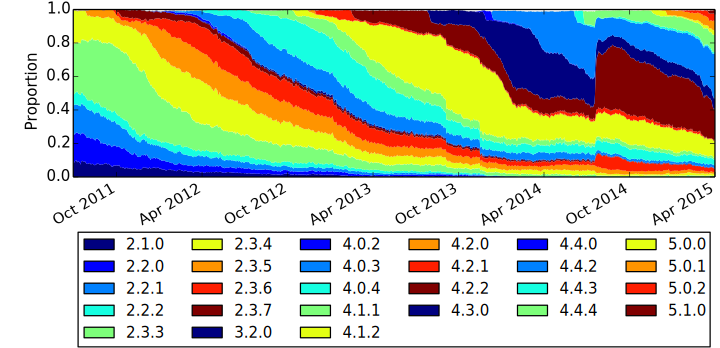
\includegraphics[width=\columnwidth]{figures/da_norm_os}
 \caption{Android versions in Device Analyzer data over time}
 \label{fig:norm_os}
\end{figure}

Figure \ref{fig:vulnerabilities} shows which vulnerabilities devices are exposed to.
For each vulnerability it shows the proportion of devices exposed to that vulnerability and how that changes over time.
In July 2011 at the beginning of the Device Analyzer data the Exploid and Levitator vulnerabilities both affect most Android devices, slowly these are fixed as updates roll out and devices are replaced until in January 2013 a much smaller proportion of devices are affected by known vulnerabilities.
However when in February 2013 the first APK signing vulnerability was found which affected all previous versions of Android and even in October 2013 most devices were still unfixed. %TODO put percentages on these things to quantify them
\begin{figure}%[!b]
\centering
\includegraphics[width=\columnwidth]{figures/vulnerabilities}
\caption{Proportion of devices exposed to each vulnerability with time (1.0 is 100\%)}
\label{fig:vulnerabilities}
\end{figure}

The variation of the proportion of devices affected by a vulnerability with time tells us how bad a particular vulnerability affected the Android platform.
Figure \ref{fig:nvulnerabilities_heat} breaks this down by vulnerability to show how the proportion of devices affected by different vulnerabilities varies.
In 2013 three vulnerabilities were found in the way which Android verified the signatures on APKs.
These allowed the creation of malicious APKs which appear to be signed as system APKs -- which have root equivalent privileges.
Figure \ref{fig:nvulnerabilities_heat} shows how the the \emph{APK signing vulnerabilities} affected all devices and took months to get fixed for any device.
However what is perhaps more worrying is the long tail on the \emph{Gingerbreak}, \emph{levitator} and \emph{exploid} vulnerabilities which are more dangerous root exploits (not requiring new APK installation) and which still affect a significant proportion of devices years later.

\begin{figure}
 \includegraphics[width=0.5\textwidth]{figures/nvulnerabilities_heat.pdf}
 \caption{Proportion of devices affected by different vulnerabilities}
 \label{fig:nvulnerabilities_heat}
\end{figure}
\begin{figure}
 \includegraphics[width=0.5\textwidth]{figures/from_to_updates.pdf}
 \caption{Updates between different Android versions in the DA data}
 \label{fig:from_to_updates}
\end{figure}
\begin{figure}
 \includegraphics[width=0.5\textwidth]{figures/w_security_updates.pdf}
 \caption{Number of updates each week which fixed or may have fixed security vulnerabilities}
 \label{fig:weekly_security_updates}
\end{figure}
Figure \ref{fig:from_to_updates} shows how devices upgrade between different versions of Android.
Device Analyzer (DA) observes upgrade events and the figure shows which versions a device is upgrading from and to.
Mostly the dark cells are above the diagonal and are upgrades.
While many upgrades are from one version to the next version there are also a fair number which skip a few versions.
Surprisingly there are also a small number of downgrade events when older versions of Android are installed on to devices.
Figure \ref{fig:weekly_security_updates} shows the number of devices getting security updates each week, blue shows updates which changed the Android version number from a version with known vulnerabilities to one which had fewer known vulnerabilities.
Red indicates updates which changed the build number but not the version number and so might contain a backported fix for a vulnerability.

\subsection{Update frequency}
%TODO find out what the frequency of updates is

\subsection{Monetisation}
One of the key differences between smartphones and desktops is that it is easier to directly cash out on a smartphone as malware can send premium rate texts or make premium rate phone calls.
It can also steal personal data which already has semantic information associated with it, this also makes it easier to perform ransomware attacks where malware deletes this information from the device and charges a ransom for its return.
It can also do more conventional things such as use the devices for DDoS attacks and altering the ads displayed to send the fees to the malware author.
While many of these things can be done by malware which just requests the relevant permissions, root exploits make this easier, particularly for ransomware and altering the ads displayed.

\subsection{Incentives and participants}
\label{sec:economics}

\section{Related work}
\label{sec:related}
Stopping root exploits working: SEAndroid, Capsicum, iOS.
Detecting malware: Android antivirus useless.


\section{Conclusion}
\label{sec:conclusion}

\printbibliography

\end{document}
